%!TEX root = ../thesis.tex
%*******************************************************************************
%*********************************** Fifth Chapter *****************************
%*******************************************************************************

\chapter{Results and Analysis}  %Title of the Fifth Chapter

\ifpdf
    \graphicspath{{Chapter1/Figs/Raster/}{Chapter1/Figs/PDF/}{Chapter1/Figs/}{/Users/luyolomagangane/Documents/Academics/Images/Recursive-Neural-Tensor-Networks/}}
\else
    \graphicspath{{Chapter1/Figs/Vector/}{Chapter1/Figs/}}
\fi


\section{Hypotheses Validation}
\dots and some more \dots
% Background on 3 hypotheses that were tested
\subsubsection{Hypothesis Overview}
In this chapter we evaluate three hypothesis explored in latent feature modelling for link prediction. Latent feature modelling has traditionally relied on linear modelling techniques in order to constrain parameterisation for computational efficiency at the expense of model expressiveness i.e. models that suffer from high bias. Recently nonlinear approaches have been proposed to overcome the bias problem and each propose hypothesis that aim to take advantage of their distinct architecture. The first nonlinear model to gain surpass state-of-the-art tensor factorisation models, was the recursive neural tensor network \cite{refefence}. There are two hypotheses proposed that were proposed in using this model architecture for link prediction, namely that recursive architectures are useful in part of speech tagging \cite{reference}, as the perform a combinatorial analysis of word sequences in sentences, instead of the conventional linear sequence used in part of speech tagging \cite{reference}. The second hypothesis is that pre-trained word embeddings offer superior performance to randomly generated entity vectors which were commonly used at the time for tensor factorisation \cite{reference}. \newline
The second hypothesis we explored is the use of convolutional hyper networks with relational factorisation for link prediction \cite{reference}. This research is the current state-of-that-art latent feature modelling technique for link prediction \cite{reference}. There are also two hypotheses explored in this research - the first is that convolutional filters can be used explicitly for relational factorisation \cite{reference}, the second is that the hyper network architecture is useful in generating the relational filters due to increased parameterisation using a hyper linear layer \cite{reference}. \newline
The final hypothesis we explored is the use of contextual entity representations as input to convolutional hyper networks. State-of-the-art natural language modelling techniques makes use contextual word representations \cite{Elmo, Bert} instead of static word embeddings \cite{fasttext, GloVe, Word2Vec}. Contextual word embeddings are represented as distinct subject entity representations, and distinct object entity representations. \newline
The following chapter presents the results and analysis from the experiments performed to validate these hypotheses.

\section{Recursive Neural Tensor Networks}
\subsubsection{Model Summary} 
Tensor factorisation has been a popular approach applied to latent feature modelling \cite{reference, reference, reference}. in order to improve model expressiveness, a Recursive Neural Tensor Network architecture was proposed \cite{reference}. This model is inspired by recursive neural networks \cite{reference}. Recursive neural networks have been applied to natural language processing tasks, particularly part of speech tagging \cite{reference}. Traditionally recurrent neural networks have been applied to this task \cite{reference}. Recurrent neural networks are based on the Markov assumption \cite{reference}, where the future states of the process depends only on the present state, not on the sequence of events that preceded it \cite{reference}. The state is constructed using sequential input within a time step window, for example, a sentence will contain a sequence of words, and the window will be the last word in the sentence and the four previous words before an anchor word. The state consists of the four previous words before the anchor word, and along with the anchor word, can be used to predict the next word in the sequence.\newline
Instead of producing a state using a sequence of previous words, recursive neural networks generate the state using a combinatorial tree of the word sequence. The number of potential combinations are dependent on the length of the sequence for example, a three word sequence has three combinations, a four word sequence has six combinations and  a five word sequence has ten combinations. The combinations which produce the smallest magnitudes are then filtered out from the network, and remaining combinations are then recombined as new combinations, This filtering and recombination process is then continued until a next word prediction is made. \newline
Recursive neural networks are combined with tensor factorisation to produce a more expressive model for link prediction. The subject and object entities are concatenated and then an matrix multiplication is taken with the resultant vector before a bias is added. \newline
\subsubsection{Contrastive Max Margin Loss}
The contrastive max-magrin loss \cite{reference} is used to train the RTNT model. The input consists of an entity-relational pair, where the entity is a subject entity. An object entity is presented as a target to complete the triple. A non-related object entity is presented is then presented as a corrupt object entity. Fact score is then computed for the target triple, as well as the corrupt triple as logits, and the difference between the two logits is the contrast between the true and false facts. The task is for the model is then to produce a higher fact score for the true triple than the false triple. If the model gets it wrong, then loss is generated and back propagated through the network to update model parameters. \newline

\subsubsection{Experimental Setup} 

We use the following benchmark datasets: Wordnet - a lexical database for English, it is a taxonomy with hypernyms (is-a) relationships, and synonym sets. Wordnet contains 38,696 entities and 11 relations.  \newline
Freebase - a large collaborative knowledge base consisting of data about the world composed mainly by its community members. It was an online collection of structured data harvested from many sources, including user-submitted wiki contributions. Freebase contains 75,043 entities and 13 relations. 
We used the Tensorflow framework to develop our model. Randomly initialised entity and relational embeddings are used to initialise model training. These embeddings are dynamically adjusted during the training process to generate latent representations specific to the knowledge domain. Model hyperparameter optimisation is implemented using random grid search. The the model was trained on a MacBook Pro 2015 with 8 cores, 16GB RAM, and 512GB SSD. \newline
We evaluate the model by ranking the accuracy scores of the predicted triples for the respective datasets. Code to reproduce: https://github.com/xhosaBoy/deep-knowledge-modelling

\subsubsection{Link Prediction Results}
The link prediction accuracy results of the RNTN model, a nonlinear factorisation model compared against linear factorisation models, are presented in table 5.1:

\begin{table}[H]
\caption{Link prediction accuracy on Wordnet and Freebase}
\centering
\begin{tabular}{lllllllllll}
  \textbf{Model} & \textbf{Wordnet} & \textbf{Freebbase} & \textbf{Avg} \\
  \hline
  Distance Model & .683 & .610 & .647 \\
  Hadamard Model & .800 & .688 & .744 \\
  Single Layer Model & .760 & .853 & .807 \\
  Bilinear Model & \textbf{.841} & \textbf{.877} & \textbf{.859} \\
  Recursive Neural Tensor Network & .732 & .518 & .625 \\

\end{tabular}
\end{table}

\subsubsection{Bias Variance Trade Off}
Machine learning models can suffer from overfitting \cite{reference} - when training has progressed too long, and the model parameters have been optimised for prediction on the training set. This leads to poor generalisation  and reveals itself in the form of increasing training accuracy, and decreasing validation accuracy. In order to overcome this problem, early stopping is often used during training. This is when triaining is terminated should decreasing validation accuracy be detected.\newline
% Hyperparameter optimisation

\begin{center}
    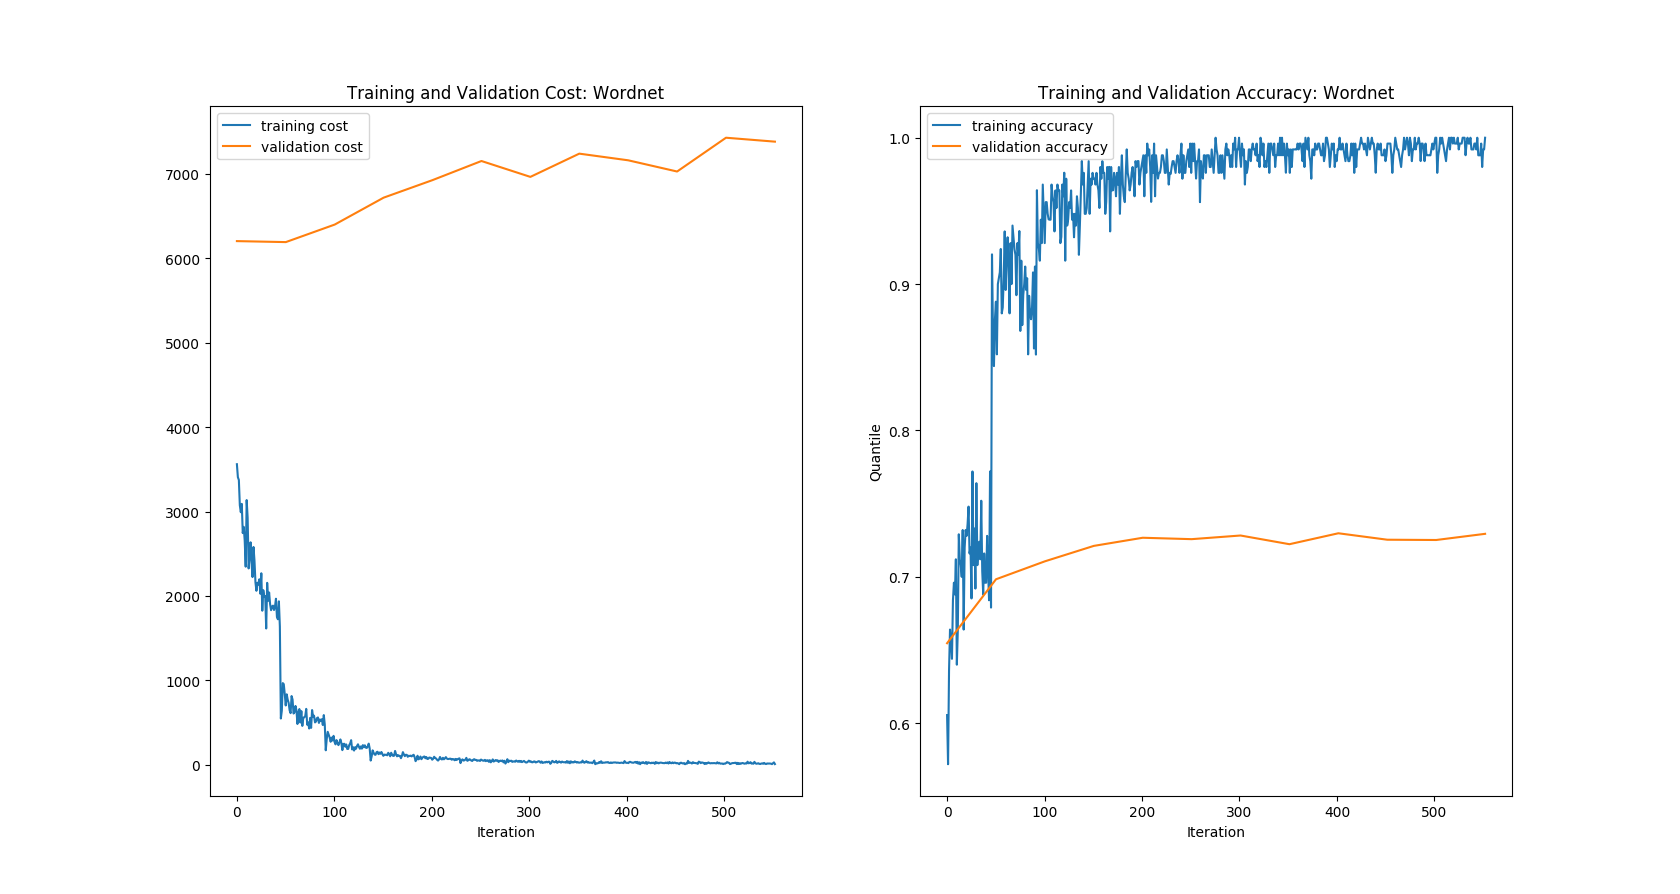
\includegraphics[width=\textwidth]{RNTN_Training_Results_Wordnet.png}
\end{center}

\begin{center}
    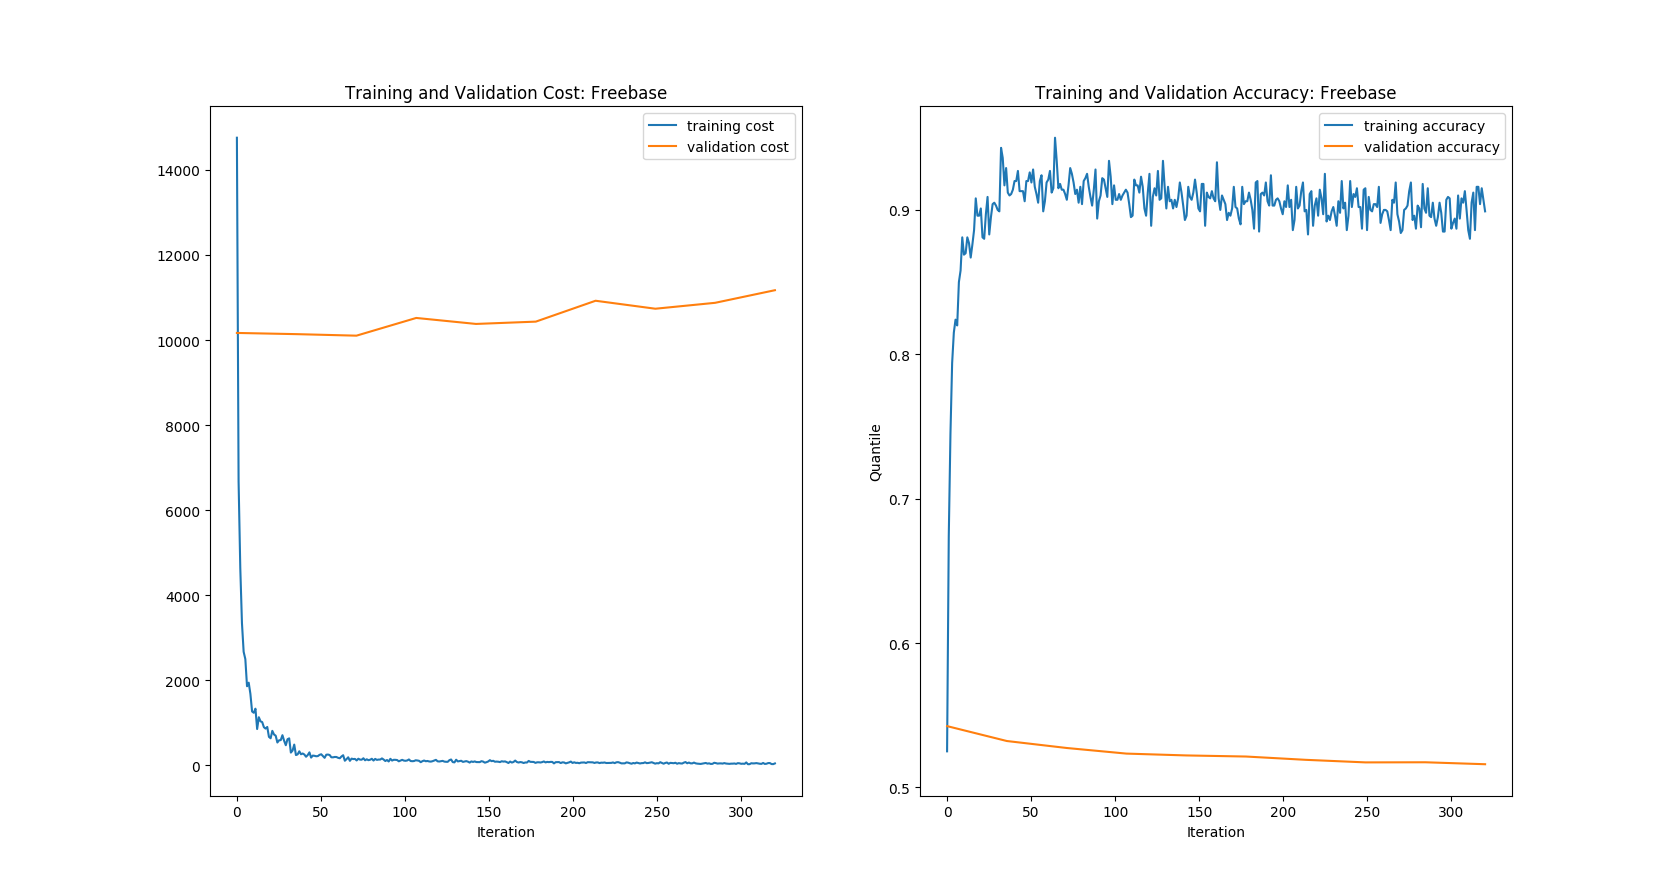
\includegraphics[width=\textwidth]{RNTN_Training_Results_Freebase.png}
\end{center}

\section{HypER Convolutional Neural Networks}

\subsubsection{Model Summary} 
In order to overcome the expressiveness problems evident in the Freebase test dataset, more nonlinear relational factorisation approaches have been proposed \cite{ComplEx, Neural LP, TorusE}. \newline
HypER is a model that uses convolutional relational filters r that are convolved with the subject entity e1, producing an intermediate relational representation. The dot product of the relational representation is then taken with the object entity e2 to produce relation-specific score between the two entities. The HypER model only produces a latent relational representation for the subject entity e1, we extend this model to also produce a relational representation for the object entity e2, and call this model HpyER+. HypER+ thus produces entity-relational representations that approximate KG spacial locality. \newline
\subsubsection{Binary Cross Entropy Loss}
The binary cross entropy loss \cite{reference} is used to train the HypER Convolutional model. Like the RNTN model, the input consists of an entity-relational pair, where the entity is a subject entity and an object entity is presented as a target to complete the triple. A logit is generated for each sample and passed through through a logarithmic sigmoid or softmax function. Loss is generated by comparing the produced likelihood with the expected likelihood, 0 or 1. The sum of all losses is aggregated and back propagated through the network for parameter update. \newline

\subsubsection{Experimental Setup} 

We use the following benchmark datasets: WN18 (Bordes et el. 2013): WN18 is a subset of Wordent, a lexical database for English, it is a taxonomy with hypernyms (is-a) relationships, and synonym sets. The dataset contains 40,943 entities and 18 relations. WN18RR (Detmers etl el. 2018): WN18RR is a subset of WN18, created by removing the inverse relations. WN18RR contains 40,943 entities and 11 relations. \newline 
FB15k (Bordes et el. 2013): FB15k is a subset of Freebase, a large collaborative knowledge base consisting of data about the world composed mainly by its community members. It was an online collection of structured data harvested from many sources, including user-submitted wiki contributions. FB15k contains 14,951 entities and 1,345 relations. FB15k-237 (Toutanova et el. 2018): FB15k-237 is a subset of FB15k, created by removing the inverse relations. WN18RR contains 40,943 entities and 11 relations. \newline
We used the PyTorch framework to develop our model. The code to reproduce results can be found on GitHub 1. Randomly initialised entity and relational embeddings are used to initialise model training. These embeddings are dynamically adjusted during the training process to generate latent representations specific to the knowledge domain. Model hyperparameter optimisation is implemented using random grid search. The the model was trained on a high-memory Google Compute Engine instance with 8 cores, 16GB RAM, 250GB SSD with a NVIDIA Tesla V100. \newline
We evaluate the model by ranking the scores of the predicted triples. Three ranking metrics are computed: Hit@10 - The percentage of predictions where the target object entity appeared within the top 10 results. Hit@3 - The percentage of predictions where the target object entity appeared within the top 3 results. Hit@1 - The percentage of predictions where the target object entity appeared as the topped ranked result. The mean rank (MR) of target the target entity object, as well as the reciprocal of the mean rank (MRR) are also computed as model evaluation metrics. Code to reproduce: https://github.com/xhosaBoy/hypernetwork-factorisation

\subsubsection{Link Prediction Results}
The link prediction accuracy results of the HypER Convolutional model, compared against other nonlinear factorisation models, are presented in table 5.2:

\begin{table}[H]
\caption{Link prediction results on WN18 and FB15k.}
\centering
\begin{tabular}{lllllllllll}
  \textbf{Dataset} & & &  \textbf{WN18} & & & & \textbf{FB15k} \\
  \hline
  & MR & MRR & H@10  & H@3  & H@1 & MR & MRR & H@10 & H@3 & H@1 \\
  \hline
  TransE & 251 & - & .892 & - & - & 125 & - & .471 & - & - \\
  DistMult & 902 & .822 & .936 & .914 & .728 & 97 & .654 & .824 & .733 & .546 \\
  ComplEx & - & .941 & .947 & .936 & .936 & - & .692 & .840 & .759 & .599 \\
  ANALOGY & - & .942 & .947 & .944 & .939 & - & .725 & .854 & .785 & .646 \\
  Neural LP & - & .940 & .945 & - & - & - & .760 & .837 & - & - \\
  R-GCN & - & .819 & .964 & .929 & .697 & - & .696 & .842 & .760 & .601 \\
  TorusE & - & .947 & .954 & .950 & .943 & - & .733 & .832 & .771 & .674 \\
  ConvE & 374  & .943 & .956 & .946 & .935 & 51 & .657 & .831 & .723 & .558 \\
  HypER & 431 & .951 & .958 & .955 & .947 & 44 & .790 & .885 & .829 & .734 \\
  HypER-BM & 434 & .941 & .952 &  .948 & .934 & 

\end{tabular}
\end{table}

% Susceptible to overfitting and early stopping solution
Machine learning models can suffer from overfitting \cite{reference} - when training has progressed too long, and the model parameters have been optimised for prediction on the training set. This leads to poor generalisation  and reveals itself in the form of increasing training accuracy, and decreasing validation accuracy. In order to overcome this problem, early stopping is often used during training. This is when triaining is terminated should decreasing validation accuracy be detected.\newline
% Hyperparameter optimisation

\begin{center}
    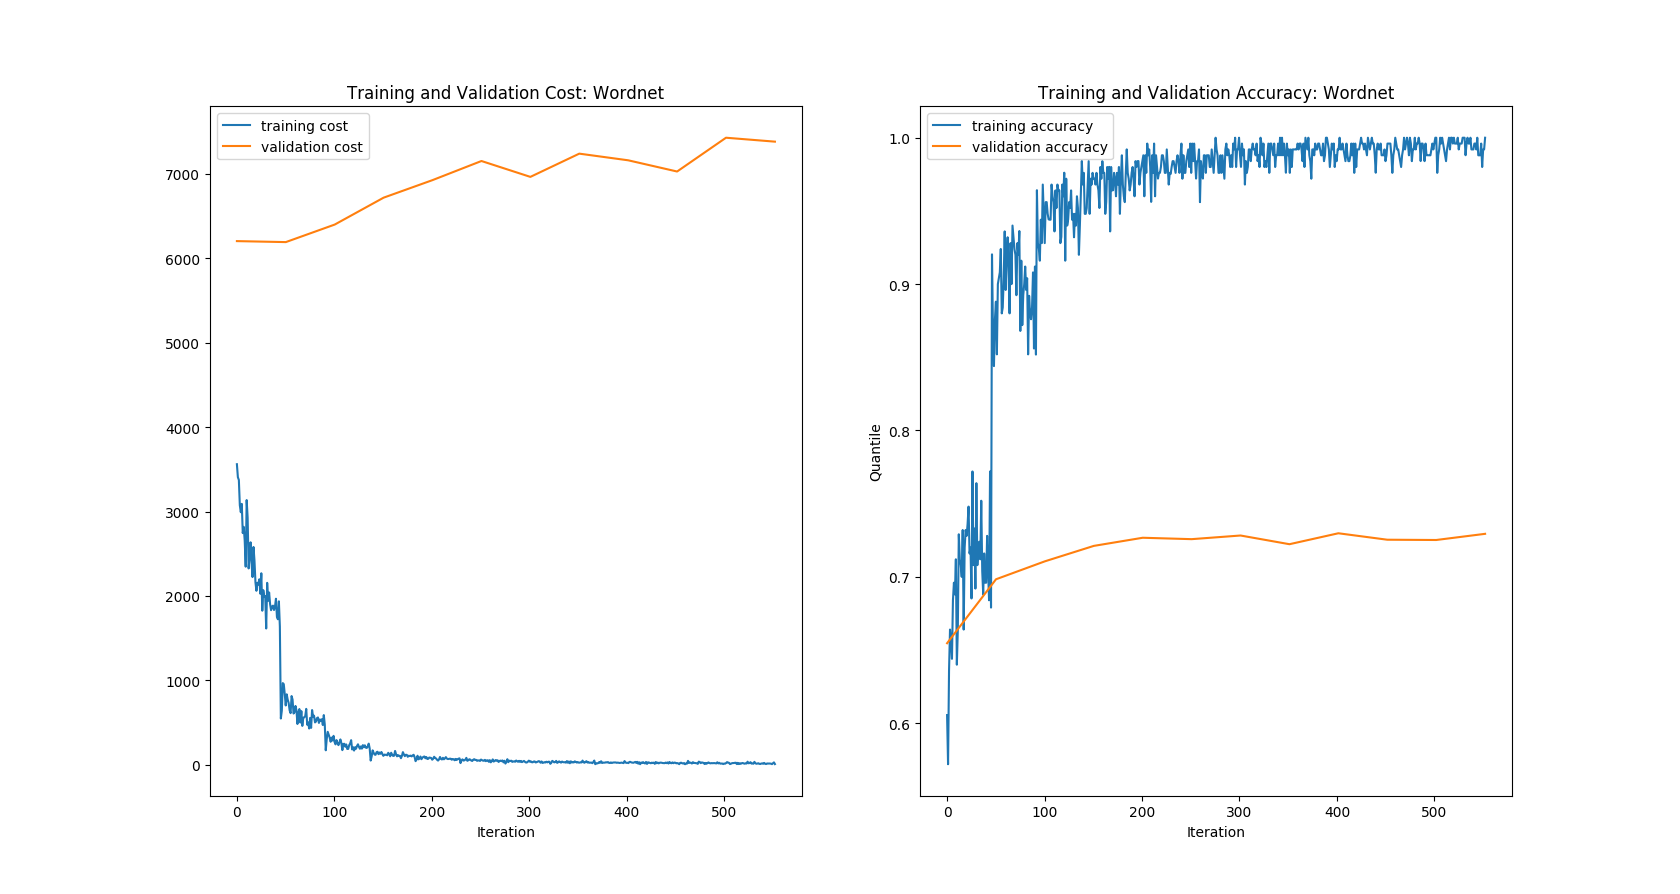
\includegraphics[width=\textwidth]{RNTN_Training_Results_Wordnet.png}
\end{center}

\begin{center}
    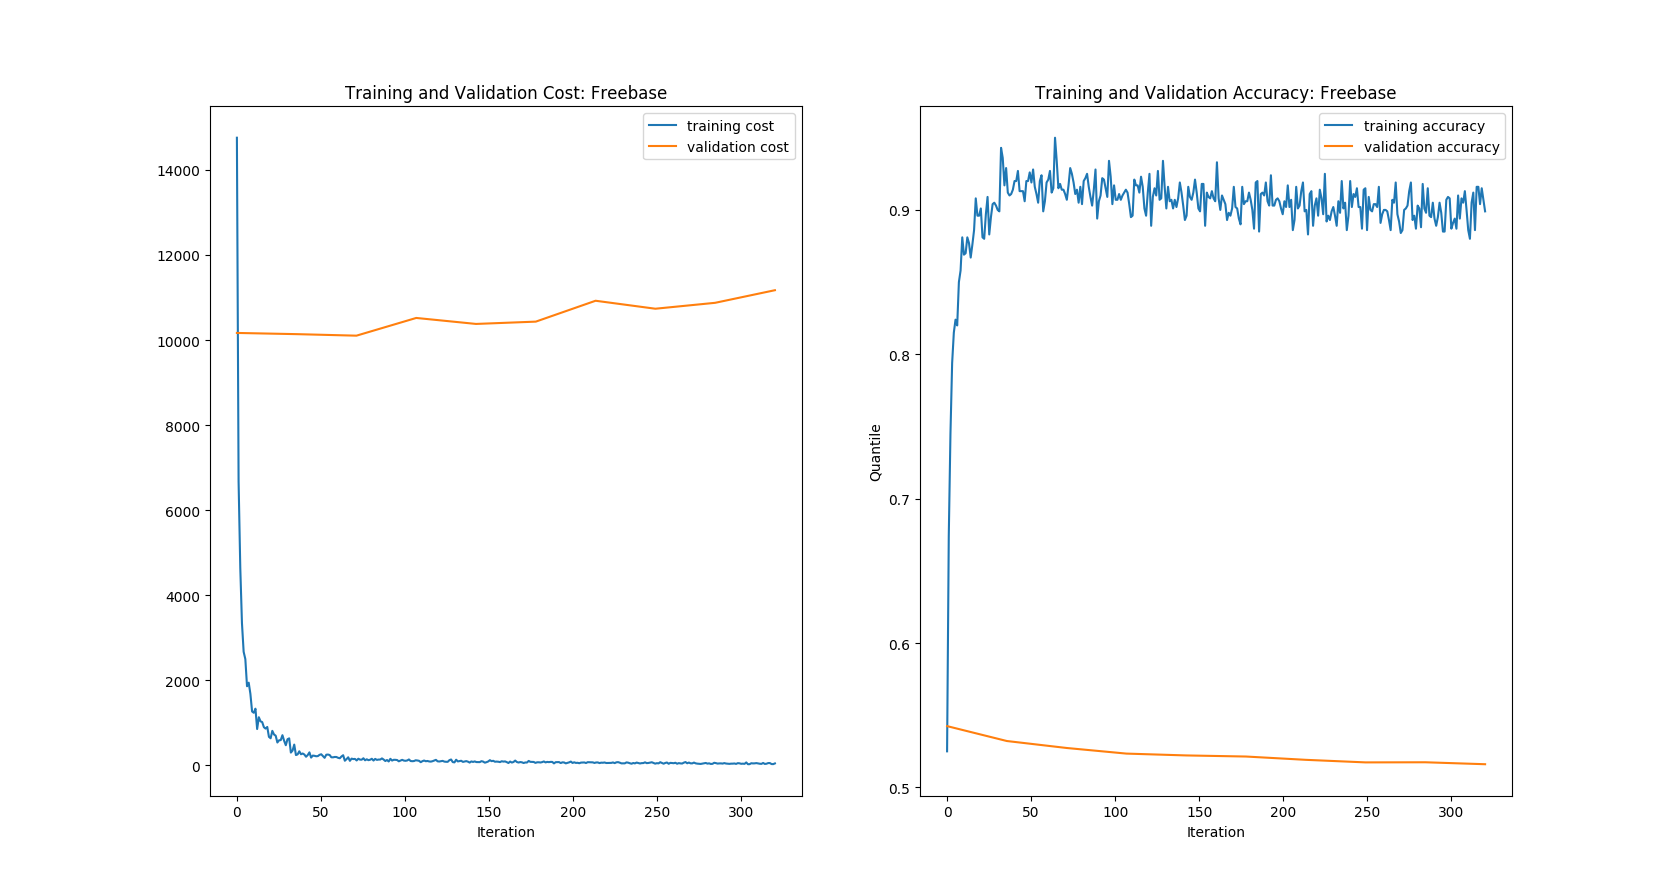
\includegraphics[width=\textwidth]{RNTN_Training_Results_Freebase.png}
\end{center}



\section{HypER Convolutional Neural Networks with Contextual Entity Embeddings}

\section{Leader Board Research Versus Hypothesis Research}

